\chapter{Continuous-Time Markov Chains}
\label{ch:ctmc}

Having explored discrete-time systems, we now turn our attention to processes that evolve continuously in time but still occupy a discrete set of states. This is a common scenario in many fields: a gene can be "on" or "off", an ion channel can be "open" or "closed", and an individual in a population can be "susceptible", "infected", or "recovered". These systems are not governed by the discrete-time transition matrix of a DTMC, but by a more dynamic framework known as the \textbf{Continuous-Time Markov Chain (CTMC)}.

\section{Fundamental Properties}

A Continuous-Time Markov Chain is a stochastic process that combines the discrete state space of a DTMC with a continuous timeline.

\begin{definitionblock}[Continuous-Time Markov Chain]
A stochastic process $\{X_t\}$, where time $t$ is continuous ($t \in \mathbb{R}^+_0$), is a \textbf{CTMC} if it satisfies:
\begin{enumerate}
    \item \textbf{Discrete State Space:} The process can only occupy states from a finite or countably infinite set $S = \{s_1, s_2, \ldots, s_N\}$.
    \item \textbf{Markov Property:} The future state of the system depends only on its present state, not on its history. For any infinitesimal time step $dt > 0$:
    $$
    P\left(X(t+dt) = \alpha \mid X(\theta) \text{ for } \theta \le t\right) = P\left(X(t+dt) = \alpha \mid X(t)\right)
    $$
\end{enumerate}
\end{definitionblock}

The core difference from DTMCs lies in how transitions are described. Instead of a matrix of one-step probabilities, CTMCs are characterized by \textbf{transition rates}. This concept is built on a set of assumptions about what can happen in an infinitesimally small time interval $dt$. These were first clarified by the physicist Wolfgang Pauli.

\begin{enumerate}
    \item \textbf{At most one event:} In an infinitesimal time interval $(t, t+dt)$, the probability of two or more transitions occurring is negligible.
    $$ P(\text{Two or more events in } (t, t+dt)) = O(dt^2) \approx 0 $$
    
    \item \textbf{Infinitesimal transition probability:} The probability of a single transition from a state $\sigma$ to a different state $\alpha$ is proportional to the duration of the interval, $dt$.
    $$ P(\text{One event in } (t, t+dt)) = O(dt) $$
\end{enumerate}

This leads to the definition of the \textbf{transition rate} (or \textbf{propensity}), $W_{\alpha\sigma}$, from state $\sigma$ to state $\alpha$:
$$
P(X(t+dt) = \alpha \mid X(t) = \sigma) = W_{\alpha\sigma} \, dt
$$
\begin{warningblock}[Rate, not Probability]
It is crucial to remember that $W_{\alpha\sigma}$ is a rate, not a probability. Its units are $1/\text{time}$. It can be greater than 1. For a transition to occur, this rate must be multiplied by the time interval $dt$.
\end{warningblock}

From these principles, we can deduce the probability of remaining in the same state. Since the sum of probabilities of transitioning from state $\sigma$ to any other state must be 1, we have:
$$
\sum_{\alpha \in S} P(X(t+dt) = \alpha \mid X(t) = \sigma) = 1
$$
Splitting the sum for the destination state $\alpha = \sigma$ and $\alpha \neq \sigma$:
$$
P(X(t+dt) = \sigma \mid X(t) = \sigma) + \sum_{\alpha \neq \sigma} P(X(t+dt) = \alpha \mid X(t) = \sigma) = 1
$$
Substituting the transition rates:
$$
P(X(t+dt) = \sigma \mid X(t) = \sigma) + \sum_{\alpha \neq \sigma} W_{\alpha\sigma} \, dt = 1
$$
Thus, the probability of no transition occurring is:
$$
P(X(t+dt) = \sigma \mid X(t) = \sigma) = 1 - \left( \sum_{\alpha \neq \sigma} W_{\alpha\sigma} \right) dt
$$

\begin{exampleblock}[The SIR Epidemic Model]
    The Susceptible-Infected-Recovered (SIR) model is a cornerstone of mathematical epidemiology and serves as a classic example of a system modeled by a CTMC. The state of the system at any time $t$ is described by the number of susceptible and infected individuas:
    
    $$
    X(t) = (S(t), I(t))
    $$
    
    In an infinitesimal time interval $dt$, two types of events can occur, each with a specific transition rate:
    
    \begin{itemize}
        \item \textbf{Infection (con):} A susceptible individual becomes infected. The state change is:
        $$ (S, I) \to (S-1, I+1) $$
        The rate of this event is proportional to the number of potential infectious contacts:
        $$ W_{\text{con}} = \beta \frac{S \cdot I}{N} $$
        where $\beta$ is the transmission rate and $N$ is the total population size.
    
        \item \textbf{Recovery (rec):} An infected individual recovers and becomes immune. The state changs:
        $$ (S, I) \to (S, I-1) $$
        The rate of recovery is proportional to the number of currently infected individuals:
        $$ W_{\text{rec}} = \gamma I $$
        where $\gamma$ is the recovery rate.
    \end{itemize}
    
    \vspace{0.5em}
    These two transition rates fully define the stochastic dynamics of the SIR model. The evolution of the probability distribution $P(S,I,t)$ is then governed by the Master Equation.
\end{exampleblock}

\section{The Master Equation}

The rules governing infinitesimal transitions allow us to derive a deterministic differential equation for the evolution of the probability distribution, $P_\sigma(t) = P(X(t)=\sigma)$: the \textbf{Master Equation}.

\subsubsection{From DTMC to CTMC: Pauli's Insight}
Before deriving the equation, let's see how the CTMC framework naturally emerges from the limit of a DTMC. Recall the Master Equation for a DTMC with discrete time steps of size $u$:
$$
P_i(t+u) = P_i(t) + \sum_{j \neq i} \left( P_j(t)\theta_{ji} - P_i(t)\theta_{ij} \right)
$$
Dividing by $u$, we get an expression resembling a time derivative:
$$
\frac{P_i(t+u) - P_i(t)}{u} = \sum_{j \neq i} \left( P_j(t)\frac{\theta_{ji}}{u} - P_i(t)\frac{\theta_{ij}}{u} \right)
$$
For this expression to converge to a meaningful limit as $u \to 0$, the transition probabilities $\theta_{ij}$ must themselves be infinitesimal and proportional to $u$. This forces us to define the transition probabilities in terms of a rate:
$$
\theta_{ij} = W_{ij} u + O(u^2)
$$
In the limit $u \to dt \to 0$, we recover the concept of a \textbf{transition rate} $W_{ij}$, and the equation becomes a differential equation.

\subsection{Derivation and Properties}
To find the probability of being in state $\sigma$ at time $t+dt$, we consider all the ways the system could have arrived there:
\begin{enumerate}
    \item The system was already in state $\sigma$ at time $t$ and did not transition out.
    \item The system was in some other state $\alpha \neq \sigma$ at time $t$ and transitioned into $\sigma$.
\end{enumerate}
Using the law of total probability, we can write:
$$
P_\sigma(t+dt) = P(X(t+dt)=\sigma \mid X(t)=\sigma)P_\sigma(t) + \sum_{\alpha \neq \sigma} P(X(t+dt)=\sigma \mid X(t)=\alpha)P_\alpha(t)
$$
Substituting the expressions for the transition probabilities:
$$
P_\sigma(t+dt) = \left( 1 - dt \sum_{\alpha \neq \sigma} W_{\alpha\sigma} \right) P_\sigma(t) + \sum_{\alpha \neq \sigma} (W_{\sigma\alpha}dt) P_\alpha(t)
$$
Rearranging the terms to find the change in probability, $P_\sigma(t+dt) - P_\sigma(t)$:
$$
\frac{P_\sigma(t+dt) - P_\sigma(t)}{dt} = \sum_{\alpha \neq \sigma} W_{\sigma\alpha} P_\alpha(t) - \left( \sum_{\alpha \neq \sigma} W_{\alpha\sigma} \right) P_\sigma(t)
$$
Taking the limit as $dt \to 0$, we arrive at the \textbf{Master Equation}:
$$
\boxed{
\dot{P}_\sigma(t) = \underbrace{\sum_{\alpha \neq \sigma} W_{\sigma\alpha} P_\alpha(t)}_{\text{Gain: Flow into } \sigma} - \underbrace{P_\sigma(t) \left( \sum_{\alpha \neq \sigma} W_{\alpha\sigma} \right)}_{\text{Loss: Flow out of } \sigma}
}
$$
This can also be written more compactly:
$$
\dot{P}_\sigma(t) = \sum_{\alpha \neq \sigma} \left( W_{\sigma\alpha}P_\alpha(t) - W_{\alpha\sigma}P_\sigma(t) \right)
$$

\subsubsection{The Fundamental Constraint: Conservation of Probability}
The Master Equation must always be complemented by the normalization constraint:
$$
\sum_{\sigma \in S} P_\sigma(t) = 1
$$
The structure of the equation ensures that if the probability is normalized at $t=0$, it remains normalized for all time. We can prove this by taking the time derivative of the total probability:
$$
\frac{d}{dt} \sum_{\sigma \in S} P_\sigma(t) = \sum_{\sigma \in S} \dot{P}_\sigma(t) = \sum_{\sigma \in S} \sum_{\alpha \neq \sigma} \left( W_{\sigma\alpha}P_\alpha(t) - W_{\alpha\sigma}P_\sigma(t) \right)
$$
The right-hand side is a double summation. We can split it into two parts:
$$
\sum_{\sigma \in S} \sum_{\alpha \neq \sigma} W_{\sigma\alpha}P_\alpha(t) - \sum_{\sigma \in S} \sum_{\alpha \neq \sigma} W_{\alpha\sigma}P_\sigma(t)
$$
In the first term, we can swap the dummy summation indices $\sigma \leftrightarrow \alpha$:
$$
= \sum_{\alpha \in S} \sum_{\sigma \neq \alpha} W_{\alpha\sigma}P_\sigma(t) - \sum_{\sigma \in S} \sum_{\alpha \neq \sigma} W_{\alpha\sigma}P_\sigma(t) = 0
$$
The two terms are identical and cancel out. Thus, the total probability is conserved.

\begin{exampleblock}[The Fundamental 2-State Irreversible CTMC]
    The simplest, yet theoretically most important, CTMC is the irreversible two-state process. It is fundamental to understanding the nature of waiting times and forms the basis of the Gillespie simulation algorithm.
    
    \begin{center}
    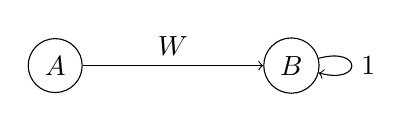
\begin{tikzpicture}
        \node[circle,draw] (A) at (0,0) {$A$};
        \node[circle,draw] (B) at (3,0) {$B$};
        \draw[->] (A) to node[above] {$W$} (B);
        \draw[->] (B) to[loop right] node[right] {$1$} (B);
    \end{tikzpicture}
    \end{center}
    
    The system has a state space $S = \{A, B\}$, where state B is \textbf{absorbing}. The only possible transition is from A to B with a constant rate $W$. The transition probabilities in an infinitesimal interval $dt$ are:
    \begin{align*}
        P(X(t+dt)=B \mid X(t)=A) &= W dt \\
        P(X(t+dt)=A \mid X(t)=A) &= 1 - W dt
    \end{align*}
    The Master Equation for the probability of being in state A, $P_A(t)$, is derived from the fact that the system can only be in state A at time $t+dt$ if it was already there at time $t$ and did not transition:
    $$
    P_A(t+dt) = P_A(t) \cdot (1 - W dt)
    \qquad \xrightarrow{dt \to 0} \qquad
    \dot{P}_A(t) = -W P_A(t)
    $$
    With an initial condition $P_A(0)$, the solution is a simple exponential decay:
    $$
    P_A(t) = P_A(0)e^{-Wt}
    $$

    A crucial question is: if the system starts in state A, how long will it stay there before jumping to B? Let $T$ be the random variable for this \textbf{permanence time}. We will see that the waiting time in any state of a CTMC is always exponentially distributed, thus:
    $$
    \langle T \rangle = \frac{1}{W}
    $$
    Intuitively, if the transition rate $W$ is high, the average waiting time is short, and vice-versa.
\end{exampleblock}

\subsection{Permanence Time and the Exponential Distribution}

A fundamental question for CTMCs is: \textit{Given that the system is in state $\sigma$ at time $t=0$, what is the probability distribution for the time $T$ until it leaves this state?}

Let $T$ be the random variable representing the \textbf{permanence time} (or waiting time) in state $\sigma$. The process can leave state $\sigma$ by making a transition to any other state $\alpha \neq \sigma$, each with rate $W_{\alpha\sigma}$. The total rate of leaving state $\sigma$ is
$$
W_{\text{out}} = \sum_{\alpha \neq \sigma} W_{\alpha\sigma}.
$$

The probability that the process remains in state $\sigma$ up to time $t$ is the \textbf{survival probability}:
$$
P_\sigma(t) = \Pr(T > t \mid X(0) = \sigma).
$$
This probability satisfies the differential equation
$$
\frac{d}{dt} P_\sigma(t) = -W_{\text{out}} P_\sigma(t),
$$
with initial condition $P_\sigma(0) = 1$. The solution is
$$
P_\sigma(t) = e^{-W_{\text{out}} t}.
$$

This is the survival function for the permanence time $T$. The CDF for $T$ is:
$$
F_T(t) = \Pr(T \leq t) = 1 - e^{-W_{\text{out}} t},
$$
and the probability density function (PDF) is
$$
\rho_T(t) = \frac{dF_T(t)}{dt} = W_{\text{out}} e^{-W_{\text{out}} t}.
$$

Thus, the permanence time in any state of a CTMC is \textbf{exponentially distributed} with parameter $W_{\text{out}}$. The mean waiting time in state $\sigma$ is
$$
\mathbb{E}[T] = \int_0^\infty t\, \rho_T(t)\,dt = \frac{1}{W_{\text{out}}}.
$$

A large $W_{\text{out}}$ means the process leaves state $\sigma$ quickly (short average waiting time), while a small $W_{\text{out}}$ means it tends to remain in $\sigma$ longer.

\subsection{Matrix Formulation}

The Master Equation for a continuous-time Markov process can be written as a system of linear ordinary differential equations (ODEs):
$$
\dot{P} = A P
$$
where $P = (P_1, \ldots, P_{|S|})^T$ is the column vector of state probabilities, and $A$ is the \textbf{transition rate matrix} (also called the \textbf{generator matrix}). The formal solution to this ODE system is:
$$
P(t) = e^{A t} P(0) = \Pi(t) P(0)
$$
where $e^{A t}$ is the matrix exponential and $\Pi(t)$ is the \textbf{transition probability matrix}, with entries:
$$
\Pi_{ij}(t) = \Pr(X(t) = i \mid X(0) = j)
$$
The Chapman-Kolmogorov Equation (CKE) states that for any $t_1, t_2 \geq 0$,
$$
\Pi(t_1 + t_2) = \Pi(t_1) \Pi(t_2)
$$
This property follows directly from the properties of the matrix exponential and encodes the Markov property: the probability of transitioning from $j$ to $i$ in time $t_1 + t_2$ is the sum over all possible intermediate states $k$ of the probability of going from $j$ to $k$ in time $t_2$ and then from $k$ to $i$ in time $t_1$.

\subsubsection{Structure of the Generator Matrix $A$}

The elements of $A$ are given by:
\begin{itemize}
    \item \textbf{Off-diagonal elements} ($i \neq j$): $A_{ij} = W_{ij}$, the transition rate from state $j$ to state $i$.
    \item \textbf{Diagonal elements}: $A_{ii} = -\sum_{k \neq i} W_{ki}$, the negative of the total rate of leaving state $i$.
\end{itemize}
Thus, each column of $A$ sums to zero:
$$
\textstyle
\sum_{i} A_{ij} = 0 \qquad \forall j
$$
This means $A$ is singular and always has an eigenvalue $\lambda = 0$. The corresponding right eigenvector $\pi$ (with $A\pi = 0$) gives the \textbf{stationary distribution} of the process,  where $\dot{P} = 0$.

\begin{exampleblock}[Another Two-State CTMC]
    Let us now consider a two-state continuous-time Markov chain (CTMC) where transitions can occur in both directions:
    
    \begin{center}
    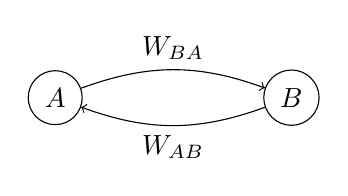
\begin{tikzpicture}
        \node[circle,draw] (A) at (0,0) {$A$};
        \node[circle,draw] (B) at (3,0) {$B$};
        \draw[->] (A) to[bend left=20] node[above] {$W_{BA}$} (B);
        \draw[->] (B) to[bend left=20] node[below] {$W_{AB}$} (A);
    \end{tikzpicture}
    \end{center}

    The system can transition from $A \to B$ with rate $W_{BA}$ and from $B \to A$ with rate $W_{AB}$. The Master Equations for the probabilities $P_A(t)$ and $P_B(t)$ of being in states $A$ and $B$ at time $t$ are:
    \begin{align*}
        \dot{P}_A(t) &= -W_{BA}P_A(t) + W_{AB}P_B(t) \\
        \dot{P}_B(t) &= -W_{AB}P_B(t) + W_{BA}P_A(t)
    \end{align*}
    Since the system must be in either $A$ or $B$ at all times, $P_A(t) + P_B(t) = 1$ thus $P_B(t) = 1 - P_A(t)$. Substituting into the first equation we get:
    \begin{align*}
        \dot{P}_A(t) &= -W_{BA}P_A(t) + W_{AB}(1 - P_A(t)) \\
        &= W_{AB} - (W_{AB} + W_{BA})P_A(t)
    \end{align*}
    At steady state ($\dot{P}_A = 0$), we solve for the stationary probability $P_A^{\mathrm{eq}}$:
    $$
    0 = W_{AB} - (W_{AB} + W_{BA})P_A^{\mathrm{eq}}
    \quad \implies \quad P_A^{\mathrm{eq}} = \frac{W_{AB}}{W_{AB} + W_{BA}}
    $$
    Similarly, for state $B$:
    $$
    P_B^{\mathrm{eq}} = 1 - P_A^{\mathrm{eq}} = \frac{W_{BA}}{W_{AB} + W_{BA}}
    $$
    The stationary distribution favors the state with the lower exit rate.

    The transition rate matrix for this process is:
    $$
    W = 
    \begin{bmatrix}
        -W_{BA} & W_{AB} \\
        W_{BA} & -W_{AB}
    \end{bmatrix}
    $$
    This matrix has rank 1, as can be verified by summing its rows. Its characteristic equation is:
    $$
    \lambda^2 + (W_{AB} + W_{BA})\lambda = 0
    $$
    which has a zero eigenvalue, guaranteeing the existence of a stationary probability distribution.
\end{exampleblock}

\subsection{Time-Varying Transition Rates}

So far, we have assumed that transition rates are constant in time, however in many cases rates can be time-dependent. Let us consider a two-state CTMC with states $A$ and $B$, where transitions are only allowed from $A$ to $B$, and the transition rate $\lambda(t)$ depends on $t$.

\begin{center}
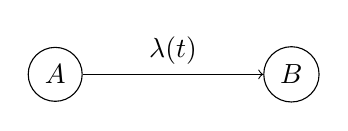
\begin{tikzpicture}
    \node[circle,draw] (A) at (0,0) {$A$};
    \node[circle,draw] (B) at (3,0) {$B$};
    \draw[->] (A) to node[above] {$\lambda(t)$} (B);
\end{tikzpicture}
\end{center}

Let $P_A(t)$ be the probability that the system is in state $A$ at time $t$. The Master Equation for $P_A(t)$ is:
$$
\dot{P}_A(t) = -\lambda(t) P_A(t)
$$
This is a first-order linear ODE with a time-dependent rate. Its solution is:
$$
P_A(t) = P_A(0) \, e^{-L(t)}
\qquad \text{where} \quad
L(t) = \int_0^t \lambda(s) ds
$$

If the system starts in state $A$ at $t=0$, then $P_A(t)$ is the probability that no transition has occurred up to time $t$. The PDF for the time $T$ of the first transition (i.e., the \textbf{permanence time} in $A$) is:
$$
\rho_T(t) = -\frac{d}{dt} P_A(t) = \lambda(t) e^{-L(t)}
$$
and the cumulative distribution function (CDF) for the waiting time is:
$$
\mathrm{CDF}_T(t) = 1 - e^{-L(t)}
$$
Thus, the probability of remaining in state $A$ up to time $t$ is $e^{-L(t)}$.

\subsubsection{The General Case: Time-Varying Matrix}

The simple two-state example can be extended. In general, the Master Equation with a time-varying transition rate matrix is:
$$
\dot{P}(t) = A(t)P(t)
$$
where the entries of the matrix $A(t)$ are unrelated functions of time. This system does not have a general analytical solution. However, we can solve it in a few important special cases.

\begin{itemize}
\item \textbf{Case 1: Separable Rates}
A solvable case occurs when all transition rates share the same time-dependent part, $\lambda(t)$. The transition matrix can be written as:
$$
A(t) = \lambda(t)\hat{A}
$$
where $\hat{A}$ is a constant matrix representing the fixed structure of the transitions. The Master Equation becomes $\dot{P}(t) = \lambda(t)\hat{A}P(t)$. By a change of time variable, this can be solved:
$$
P(t) = e^{L(t)\hat{A}} P(0)
\qquad \text{where} \quad
L(t) = \int_0^t \lambda(s)ds
$$

\item \textbf{Case 2: Piecewise-Constant Periodic Rates}
Another important and tractable case is when the matrix $A(t)$ is piecewise constant and periodic. This is common in systems subject to seasonal or diurnal forcing. For example, consider a system with period $Q$ where the dynamics are governed by matrix $A_1$ for a duration $T_1$ and then by matrix $A_2$ for a duration $T_2 = Q-T_1$.

$$
A(t) = 
\begin{cases}
    A_1 & \text{if } 0 < \text{mod}(t,Q) \le T_1 \\
    A_2 & \text{if } T_1 < \text{mod}(t,Q) \le Q
\end{cases}
$$
We can solve this system by integrating it over each constant interval.
\begin{itemize}
    \item For the first interval $0 < t \le T_1$:
    $$ \dot{P} = A_1 P \quad \implies \quad P(t) = e^{A_1 t}P(0) $$
    The state at the end of this interval is $P(T_1) = e^{A_1 T_1}P(0)$.

    \item For the second interval $T_1 < t \le Q$:
    $$ \dot{P} = A_2 P \quad \implies \quad P(t) = e^{A_2 (t-T_1)}P(T_1) $$
    The state at the end of one full period is:
    $$ P(Q) = e^{A_2 (Q-T_1)}P(T_1) = e^{A_2 T_2}e^{A_1 T_1}P(0) $$
\end{itemize}
We can define a \textbf{one-period evolution matrix} $B = e^{A_2 T_2}e^{A_1 T_1}$. The state of the system at integer multiples of the period $Q$ is then given by:
$$
P(nQ) = B^n P(0)
$$
This reduces the long-term continuous dynamics to a discrete-time evolution based on the matrix $B$. The stability and asymptotic behavior of the system are determined by the eigenvalues of $B$.
\end{itemize}

\section{The Gillespie Algorithm}
While the Master Equation describes the evolution of the probability distribution, it quickly becomes intractable for systems with many states. To study the behavior of a single realization of a CTMC, we use a simulation method that is exact, not an approximation: the \textbf{Gillespie Algorithm}.

The algorithm is based on the properties of permanence time we just derived. At any given time $t_n$, when the system is in state $X(t_n) = \sigma$, we need to answer two questions:
\begin{enumerate}
    \item \textbf{When} will the next transition occur?
    \item \textbf{Which} transition will it be?
\end{enumerate}

\begin{figure}[H]
    \centering
    \begingroup
    \small
    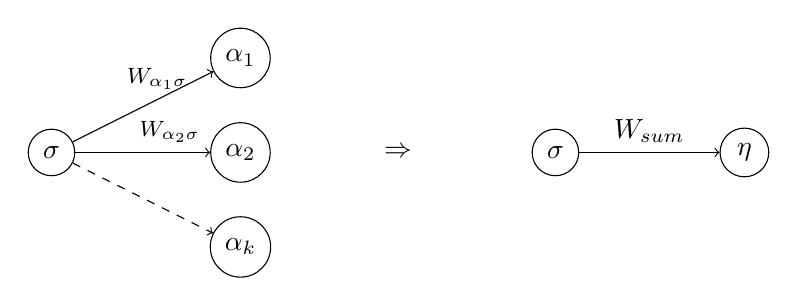
\begin{tikzpicture}[scale=0.8]
        \node[circle,draw] (s1) at (0, 0) {$\sigma$};
        \node[circle,draw] (s2) at (3, 1.5) {$\alpha_1$};
        \node[circle,draw] (s3) at (3, 0) {$\alpha_2$};
        \node[circle,draw] (s4) at (3, -1.5) {$\alpha_k$};
        \draw[->] (s1) to node[above, pos=0.6] {\footnotesize $W_{\alpha_1 \sigma}$} (s2);
        \draw[->] (s1) to node[above, pos=0.7] {\footnotesize $W_{\alpha_2 \sigma}$} (s3);
        \draw[->, dashed] (s1) to (s4);
        
        \node at (5.5, 0) {$\Rightarrow$};
        
        \node[circle,draw] (s5) at (8, 0) {$\sigma$};
        \node[circle,draw] (s6) at (11, 0) {$\eta$};
        \draw[->] (s5) to node[above] {$W_{sum}$} (s6);
    \end{tikzpicture}
    \endgroup
    \caption{From state $\sigma$, the system can jump to multiple other states. This is equivalent to a single jump to a "rest of the world" state $\eta$ with a total rate $W_{sum}$.}
\end{figure}

The key insight is that the waiting time $T$ for the \textit{next} event, regardless of which one it is, is exponentially distributed with a rate equal to the sum of all possible exit rates from the current state $\sigma$:
$$
W_{sum} = \sum_{\alpha \neq \sigma} W_{\alpha\sigma}
$$
Once we know that an event has occurred, the probability that it was a specific transition to state $\alpha_i$ is proportional to its individual rate:
$$
P(\text{Jump to } \alpha_i \mid \text{A jump occurred}) = \frac{W_{\alpha_i\sigma}}{W_{sum}}
$$
This leads to a simple and elegant simulation procedure.

\begin{algorithm}[H]
\caption{The Gillespie Algorithm (Direct Method)}
\begin{algorithmic}[1]
\State \textbf{Initialize} the system at time $t=0$ with an initial state $X(0)$. Set a final time $T_{final}$.
\While{$t < T_{final}$}
    \State Let the current state be $\sigma = X(t)$.
    \State \textbf{Calculate rates:} Compute all possible transition rates $W_{\alpha\sigma}$ out of state $\sigma$.
    \State \textbf{Calculate total rate:} Compute the sum of all rates, $W_{sum} = \sum_{\alpha} W_{\alpha\sigma}$.
    \If{$W_{sum} = 0$}
        \State The system is in an absorbing state. \textbf{break} the loop.
    \EndIf
    \State \textbf{Sample waiting time:} Draw a random number $u_1 \sim \text{U}(0,1)$. Calculate the waiting time $$T = -\frac{\ln(u_1)}{W_{sum}}$$
    \State \textbf{Sample next event:} Draw a second random number $u_2 \sim \text{U}(0,1)$. Find the event $\alpha_j$ s.t.
    $$ \frac{\sum_{k=1}^{j-1} W_{\alpha_k\sigma}}{W_{sum}} < u_2 \le \frac{\sum_{k=1}^{j} W_{\alpha_k\sigma}}{W_{sum}} $$
    \State \textbf{Update:} Set the new time $t \gets t+T$ and the new state $X(t) \gets \alpha_j$.
    \State \textbf{Record} the state and time if desired.
\EndWhile
\end{algorithmic}
\end{algorithm}

\subsection{Simulation with Time-Varying Rates}

When rates $W_{\alpha\sigma}(t)$ depend on time, simulating the process becomes more complex because the waiting time for the next event is no longer exponentially distributed. If the system is in state $\sigma$ at time $t_n$, we must find the time $T$ to the next event.

The probability of remaining in state $\sigma$ until time $t_n+T$ is:
$$
P(\text{no event in } [t_n, t_n+T]) = \exp\left( -\int_{t_n}^{t_n+T} W_{sum}(t)dt \right)
$$
where $W_{sum}(t) = \sum_{\alpha \neq \sigma} W_{\alpha\sigma}(t)$ is the time-dependent total exit rate. To sample the waiting time $T$ using the inverse transform method, we draw a random number $u \sim \text{U}(0,1)$ and solve the following integral equation for $T$:
$$
\int_{t_n}^{t_n+T} W_{sum}(t)dt = -\ln(u)
$$
This equation often has no analytical solution and must be solved numerically (e.g., using Newton's method) for $T$ at each step of the simulation. Once $T$ is found, the choice of the next event proceeds as before, using the rates evaluated at the time of the jump, $t_n+T$:
$$
P(\text{Jump to } \alpha_i) = \frac{W_{\alpha_i\sigma}(t_n+T)}{W_{sum}(t_n+T)}
$$

\begin{exampleblock}[Gillespie Simulation of the SIR model]
    Let's apply the Gillespie algorithm to the stochastic SIR model. The state of the system is given by the tuple $(S, I)$. There are two possible events that can occur from any given state $(S_n, I_n)$ at time $t_n$:
    \begin{itemize}
        \item \textbf{Infection (con):} An infected individual transmits the disease to a susceptible one:
        $$(S, I) \to (S-1, I+1), \quad W_{\text{con}} = \beta \frac{S_n I_n}{N}$$
        \item \textbf{Recovery (rec):} An infected individual recovers:
        $$(S, I) \to (S, I-1), \quad W_{\text{rec}} = \gamma I_n$$
    \end{itemize}
    
    The simulation proceeds step-by-step as follows:
    \begin{enumerate}
        \item At time $t_n$ with state $(S_n, I_n)$, calculate the two rates, $W_{\text{con}}$ and $W_{\text{rec}}$.
        \item Calculate the total exit rate: $W_{sum} = W_{\text{con}} + W_{\text{rec}}$.
        \item Draw a random number $u_1 \sim \text{Unif}(0,1)$ and determine the time to the next event:
        $$ T_n = -\frac{\ln(u_1)}{W_{sum}} $$
        The next event will occur at time $t_{n+1} = t_n + T_n$.
        \item Draw a second random number $u_2 \sim \text{Unif}(0,1)$ to determine which event occurs. The probability of a contagion event is:
        $$ P(\text{con}) = \frac{W_{\text{con}}}{W_{sum}} = \frac{\beta S_n I_n / N}{\beta S_n I_n / N + \gamma I_n} $$
        \item If $u_2 < P(\text{con})$, the event is an infection, and the state is updated to $(S_n-1, I_n+1)$. Otherwise, the event is a recovery, and the state becomes $(S_n, I_n-1)$.
        \item Repeat the process until the epidemic ends ($I=0$).
    \end{enumerate}
    
    \subsubsection*{Extension: Periodic Contact Rate}
    Now consider a more realistic scenario where the contact rate varies periodically, for example, due to seasonality:
    $$
    \beta(t) = \beta_m (1 + a \cos(\omega t))
    $$
    In this case, sampling the waiting time $T$ requires solving the integral equation:
    $$
    L(T) = \int_{t_n}^{t_n+T} W_{sum}(s)ds = -\ln(u_1)
    $$
    Given the state $(S_n, I_n)$, the sum of rates is $W_{sum}(s) = \gamma I_n + \beta(s) S_n I_n / N$. The integral $L(T)$ becomes:
    $$
    L(T) = T\gamma I_n + \frac{I_n S_n \beta_m}{N} \left( T + \frac{a}{\omega}(\sin(\omega(t_n+T)) - \sin(\omega t_n)) \right)
    $$
    This transcendental equation for $T$ must be solved numerically at each step of the simulation. Once $T$ is found, the choice of which event occurred is made by comparing $u_2$ to the ratio of the rates evaluated at the new time $t_n+T$.
    \end{exampleblock}

\section{Special Processes and Extensions}

\subsection{The Poisson Process}
The Poisson process is a fundamental CTMC that models the counting of events occurring at a constant rate $\lambda$. Let $P_n(t)$ be the probability of having observed $n$ events by time $t$. The system can only transition from state $n$ to state $n+1$.

\begin{center}
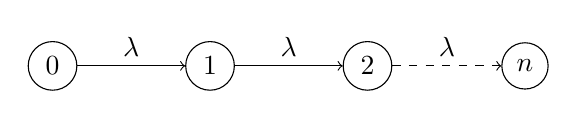
\begin{tikzpicture}
    \node[circle,draw] (s0) at (0,0) {$0$};
    \node[circle,draw] (s1) at (2,0) {$1$};
    \node[circle,draw] (s2) at (4,0) {$2$};
    \node[circle,draw] (s3) at (6,0) {$n$};
    \draw[->] (s0) to node[above]{$\lambda$} (s1);
    \draw[->] (s1) to node[above]{$\lambda$} (s2);
    \draw[->, dashed] (s2) to node[above]{$\lambda$} (s3);
\end{tikzpicture}
\end{center}

The transition rates are $W_{n+1, n} = \lambda$ for all $n \ge 0$. The Master Equation for state $n$ is:
$$
\begin{cases}
\dot{P}_n(t) = \lambda P_{n-1}(t) - \lambda P_n(t) & n \ge 1\\
\dot{P}_0(t) = -\lambda P_0(t) & n = 0
\end{cases}
$$
With the initial condition $P_0(0)=1$ (zero events at time zero), this system of ODEs can be solved recursively. The solution is the famous \textbf{Poisson distribution}:
$$
P_n(t) = \frac{(\lambda t)^n}{n!}e^{-\lambda t}
$$
\subsubsection{Poisson Process with Time-Varying Rate}
If the rate of events $\lambda(t)$ is time-dependent, the Master Equation becomes $\dot{P}_n(t) = \lambda(t) P_{n-1}(t) - \lambda(t) P_n(t)$. The solution is a generalization known as the non-homogeneous Poisson process, where the distribution at time $t$ is:
$$
P_n(t) = \frac{L(t)^n}{n!}e^{-L(t)}, \quad \text{where} \quad L(t) = \int_0^t \lambda(s)ds
$$
Here, the number of events follows a Poisson distribution with a mean equal to $L(t)$.

\subsection{Pure Death Process}
Consider a system of $N$ identical, independent particles at $t=0$, where each particle has a constant rate of decay $\gamma$. Let $X(t)=n$ be the number of particles remaining at time $t$. This is a \textbf{pure death process}, a special case of the birth-death process where the birth rate is zero. The only possible transition is from state $n$ to $n-1$. Since each of the $n$ particles can decay independently, the total rate of leaving state $n$ is:
$$
d(n) = n\gamma
$$
The Master Equation for the probability $P_n(t)$ is:
$$
\dot{P}_n(t) = (n+1)\gamma P_{n+1}(t) - n\gamma P_n(t)
$$
with the boundary condition $\dot{P}_N(t) = -N\gamma P_N(t)$. While solving this system for $P_n(t)$ is possible, it is often more insightful to study the evolution of the moments.

\subsubsection{Evolution of the Mean}
The mean number of particles is $\langle n(t) \rangle = \sum_{n=0}^N n P_n(t)$. Its time derivative is:
$$
\frac{d\langle n \rangle}{dt} = \sum_{n=0}^N n \dot{P}_n(t) = \gamma \sum_{n=0}^N n \left[ (n+1) P_{n+1} - n P_n \right]
$$
This can be split into two sums. By re-indexing the first sum ($k=n+1$), we find that the terms nearly cancel, leading to a simple ODE for the mean:
$$
\frac{d\langle n \rangle}{dt} = -\gamma \sum_{n=0}^N n P_n(t) = -\gamma \langle n(t) \rangle
$$
With the initial condition $\langle n(0) \rangle = N$, the solution is:
$$
\langle n(t) \rangle = N e^{-\gamma t}
$$
The average number of particles decays exponentially, just like in a deterministic model.

\subsubsection{Evolution of the Second Moment}
Similarly, we can find an equation for the second moment, $\langle n^2(t) \rangle$:
$$
\frac{d\langle n^2 \rangle}{dt} = \sum_{n=0}^N n^2 \dot{P}_n(t) = \gamma \sum_{n=0}^N n^2 \left[ (n+1) P_{n+1} - n P_n \right]
$$
After careful re-indexing and algebraic manipulation (using the identity $n^2 = (n+1)^2 - 2(n+1) + 1$), this simplifies to:
$$
\frac{d\langle n^2 \rangle}{dt} = -2\gamma \langle n^2(t) \rangle + \gamma \langle n(t) \rangle
$$
Substituting the known solution for $\langle n(t) \rangle$:
$$
\frac{d\langle n^2 \rangle}{dt} = -2\gamma \langle n^2 \rangle + \gamma N e^{-\gamma t}
$$
This is a linear first-order ODE for $\langle n^2 \rangle$. With the initial condition $\langle n^2(0) \rangle = N^2$, its solution is:
$$
\langle n^2(t) \rangle = N(N-1)e^{-2\gamma t} + N e^{-\gamma t}
$$
From this, we can find the variance:
$$
\text{Var}[n(t)] = \langle n^2(t) \rangle - \langle n(t) \rangle^2 = N e^{-\gamma t}(1 - e^{-\gamma t})
$$
The variance starts at zero, increases to a maximum, and then decays back to zero as all particles eventually disappear.

\subsection{Birth-Death Processes}
A particularly important class of CTMCs is the \textbf{birth-death process}, which models populations where the state $n$ (the population size) can only change by $\pm 1$. These processes are defined by two state-dependent rates:
\begin{itemize}
    \item \textbf{Birth rate $b(n)$:} The rate of transition from state $n$ to $n+1$.
    \item \textbf{Death rate $d(n)$:} The rate of transition from state $n$ to $n-1$. It is typically assumed that $d(0)=0$.
\end{itemize}
The Master Equation for the probability $P_n(t)$ of being in state $n$ is:
$$
\dot{P}_n = b(n-1)P_{n-1} + d(n+1)P_{n+1} - (b(n)+d(n))P_n
$$
\subsubsection{Steady-State Analysis}
At steady state ($\dot{P}_n=0$), the probability distribution is constant. This implies that the net flow of probability between any two adjacent states must be zero. Let's define the \textbf{probability current} $J_n$ as the net flow from state $n-1$ to $n$:
$$
J_n = b(n-1)P_{n-1} - d(n)P_n
$$
The steady-state Master Equation can be rewritten as $J_{n+1} - J_n = 0$, which means the current must be constant for all $n$. For systems with a reflective boundary at $n=0$ (no negative population), this constant must be zero. Therefore, at steady state:
$$
J_n = 0 \quad \implies \quad d(n)P_n = b(n-1)P_{n-1}
$$
This gives a simple recurrence relation for the stationary distribution $P_n$:
$$
P_n = \frac{b(n-1)}{d(n)} P_{n-1}
$$
By iterating this relation, we can express any $P_n$ in terms of $P_0$:
$$
P_n = P_0 \prod_{k=1}^{n} \frac{b(k-1)}{d(k)}
$$
The value of $P_0$ is then found by imposing the normalization condition $\sum_{n=0}^{\infty} P_n = 1$.

\begin{exampleblock}[Immigration-Death Process]
Consider a population with a constant immigration rate (birth rate) $b(n) = b$ and a per-capita death rate $d(n) = k n$. The steady state recurrence is:
$$
P_n = \frac{b}{kn}P_{n-1}
$$
Let's define $R = b/k$. The recurrence becomes $P_n = \frac{R}{n}P_{n-1}$. Iterating this:
$$
P_n = \frac{R}{n} \cdot \frac{R}{n-1}P_{n-2} = \ldots = \frac{R^n}{n!} P_0
$$
To normalize, we sum over all $n$:
$$
\sum_{n=0}^{\infty} P_n = P_0 \sum_{n=0}^{\infty} \frac{R^n}{n!} = P_0 e^R = 1 \quad \implies \quad P_0 = e^{-R}
$$
The stationary distribution is a Poisson distribution with mean $R$:
$$
P_n = \frac{R^n}{n!}e^{-R}
$$
If $R \le 1$, the distribution is monotonically decreasing. If $R > 1$, it is unimodal, with its peak near $R$.
\end{exampleblock}

% add PCTMC

\section{Population Continuous Time Markov Chains (PCTMC)}

If the state variables represent a population (of humans, of animals, of molecules, of objects etc.) then it is possible to specialize the theoretical apparatus we have developed. To start:

$$
\text{Prob}\left( x(t + dt) = \alpha|x(t) = \delta \right) = W_{\alpha\delta}dt
$$

can be rewritten (thanks to the structure of $\mathbb{N}^M_0$) as:

$$
\text{Prob}\left( x(t + dt) = \delta + (\alpha - \delta)|x(t) = \delta \right) = W_{\alpha\delta}dt
$$

Setting 
$$
V_{\alpha\delta} = (\alpha - \delta),
$$

which specifies the jump needed to switch state from $\delta$ to $\alpha$
$$
\text{Prob}\left( x(t + dt) = x(t) + V_{\alpha\delta}|x(t) = \delta \right) = W_{\alpha\delta}dt
$$

In this context, we use the index $\eta$ to label the different types of events that can occur in the system. Each event $\eta$ is defined by a specific change (or "jump") in the system's state, and occurs at a rate that generally depends on the current state.

A key feature of Population Continuous Time Markov Chains (PCTMC) is that there are only a finite number of possible events, each associated with a fixed jump vector (independent of the current state), but with a rate that depends on the current state $x(t)$:
$$
\text{Prob}\left( \text{Event}_\eta \mid x(t) \right) = \text{Prob}\left( x(t + dt) = x(t) + V^{(\eta)} \mid x(t) \right) = r_\eta(x(t))\,dt
$$
This is a restatement of the general CTMC rule, but here the focus is on events, and the fact that, in population models, event rates depend on the current state.

Let's formally define a PCTMC as:

\begin{definitionblock}[Population Continuous Time Markov Chain (PCTMC)]
A PCTMC is defined by a tuple:

\vspace{-1em}

$$
X = (X, X_0, S, T)
$$

\vspace{-1em}

where:
\begin{itemize}
    \item $S \subseteq \mathbb{N}^M_0$ is the state space (e.g., all possible population counts),
    \item $X, X_0 \in S$ are the current and initial states,
    \item $T = \{ (\text{Name}_\eta, v_\eta, r_\eta(X; t)) \}_{\eta=1}^Z$ is the set of transitions, where:
    \begin{itemize}
        \item $\text{Name}_\eta$ is the name of event $\eta$,
        \item $v_\eta \in S$ is the jump vector for event $\eta$,
        \item $r_\eta(X; t) \geq 0$ is the rate of event $\eta$, which may depend on the current state $X$ and time $t$.
    \end{itemize}
\end{itemize}

\vspace{0.5em}

The rate $r_\eta(X; t)$ must be zero if the resulting state would fall outside the state space:
$$
(X + v_\eta) \notin S \implies r_\eta(X; t) = 0.
$$
\end{definitionblock}

With this structure, the Master Equation for the probability $P_x(t)$ of being in state $x$ at time $t$ becomes:
$$
\dot{P}_x(t) = \sum_{\eta} \left[ r_\eta(x - v_\eta) P_{x - v_\eta}(t) - r_\eta(x) P_x(t) \right]
$$
This form of the Master Equation is commonly known as the \textit{Chemical Master Equation}.

\section{Approximating PCTMC Dynamics with ODEs}

A stochastic model described by a PCTMC can often be approximated by a deterministic ODE system, provided the event rates and state variables scale appropriately with a large parameter $N$ (such as population size, volume, or area). Specifically, we require that the rates satisfy:
$$
r_\eta(X; t) = N\, r_\eta\left(\frac{X}{N}; t\right)
$$
where $X$ is the state and $r_\eta$ is the rate of event $\eta$.

Define the normalized state variable $y = X/N$. The average dynamics of the system are then given by the cauchy problem:
$$
\begin{cases}
\dot{y}(t) = \sum_\eta v_\eta\, r_\eta(y; t)\\
y(0) = \frac{X(0)}{N}
\end{cases}
$$

Kurtz's theorem formalizes this approximation: for any $\delta > 0$,
$$
\lim_{N \to \infty} \Pr\left( \left| y(t) - \frac{X(t)}{N} \right| > \delta \right) = 0
$$
That is, as $N$ becomes large, the normalized stochastic process $\frac{X(t)}{N}$ converges in probability to the deterministic solution $y(t)$.

We can express the deviation as
$$
\frac{X(t)}{N} = y(t) + \varepsilon^{(N)}(t)
$$
where, for large $N$, the fluctuations $\varepsilon^{(N)}(t)$ are small:
$$
|\varepsilon^{(N)}(t)| = O(1/\sqrt{N}) \ll 1
$$

\begin{exampleblock}[ODE Approximation of the SIR model]
Recall that the deterministic SIR model is governed by the following ODEs:
$$
    \dot{S} = -\beta \frac{S I}{N}, 
    \quad 
    \dot{I} = \beta \frac{S I}{N} - \gamma I, 
    \quad
    \dot{R} = \gamma I
$$
where $S$, $I$, and $R$ represent the numbers of susceptible, infected, and recovered individuals.

As we've seen, the SIR model involves two types of events: infection (contagion) and recovery. The rates at which these events occur both scale with the total population size $N$:
\begin{align*}
    r_{\text{con}}(S, I) &= \beta \frac{1}{N} S I = N \beta \frac{S}{N} \frac{I}{N} = N r_{\text{con}}\left(\frac{S}{N}, \frac{I}{N}\right) \\
    r_{\text{rec}}(S, I) &= \gamma I = N \gamma \frac{I}{N} = N r_{\text{rec}}\left(\frac{I}{N}\right)
\end{align*}

Defining the normalized variables
$$
(y_S, y_I) = \left( \frac{S}{N}, \frac{I}{N} \right),
$$
for large $N$ the PCTMC is very well approximated by the ODE system
$$
\dot{y}_S = -\beta y_S y_I, \qquad \dot{y}_I = \beta y_S y_I - \gamma y_I.
$$

\end{exampleblock}

\subsection{The Second Gillespie Algorithm (First Reaction Method)}

Gillespie also proposed a second exact simulation algorithm, often called the \textbf{First Reaction Method}. This approach is particularly natural for Population Continuous-Time Markov Chains (PCTMCs) and is based on the idea of independently sampling the waiting time for each possible event.

\begin{enumerate}
    \item For each possible event $\eta$, sample an independent uniform random variable:
    $$
    u_\eta \sim \text{Unif}([0,1])
    $$
    \item For each event, compute its tentative firing time:
    $$
    \tau_\eta = \frac{-\log(1 - u_\eta)}{r_\eta(x(t_n))}
    $$
    where $r_\eta(x(t_n))$ is the propensity (rate) of event $\eta$ given the current state $x(t_n)$.
    \item The next event to occur is the one with the smallest $\tau_\eta$:
    $$
    \eta^* = \operatorname{ArgMin}_\eta \{\tau_\eta\}
    $$
    \item The time of the next event is:
    $$
    t_{n+1} = t_n + \tau_{\eta^*}
    $$
    \item Update the system state according to event $\eta^*$, and repeat the procedure.
\end{enumerate}

\vspace{0.5em}

This method is mathematically equivalent to the Direct Method, but can be more intuitive in some settings, as it treats each possible event as a competing exponential clock and simply executes the one that rings first.

\subsection{The Tau-Leaping Algorithm and Other Approximations}

A notable result of the PCTMC framework is that the state at time $t$ can be written as:
$$
x(t) = x(0) + \sum_\eta V_\eta \cdot K_\eta(t,0)
$$
where $K_\eta(t,0)$ represents the number of occurrences of event type $\eta$ in the time interval $(0,t)$.

More compactly, we define:
$$
K_\eta(t,dt) = \text{(\# events of type } \eta \text{ in } (t,t+dt))
$$
Since the probability of occurrence of an event of type $\eta$ in the interval $(t,t+dt)$ is $r_\eta(x(t))dt$, and this probability depends on the state variable $x(t)$, the formula above is practically unusable in its current form because $x(t)$ will stochastically depend on the history of events itself.

Indeed, following the formal proof of Theorem 1.22 in Chapter 1 of Anderson and Kurtz's book \textit{Stochastic Analysis of Biochemical Systems} (Springer, 2015), we have:
$$
K_\eta(t,0) = \text{Poisson}\left(\int_0^t r_\eta(x(s))ds\right)
$$
Daniel Gillespie, observing that:
$$
x(t+\tau) = x(t) + \sum_\eta V_\eta K_\eta(t+\tau,t)
$$
and that for small $\tau$, the equation above can be straightforwardly approximated as:
$$
K_\eta(t+\tau,t) \approx \text{Poisson}\left(\tau r_\eta(x(t))\right)
$$
proposed the following approximated simulation algorithm:
$$
x(t+\tau) \approx x(t) + \sum_\eta V_\eta \text{Poisson}\left(\tau r_\eta(x(t))\right)
$$
This is termed the \textbf{tau-leaping algorithm}.
This approximation is appropriate only when all state variables are sufficiently large. Otherwise, some populations may become negative, violating the requirement that they remain non-negative. The method also assumes that the rates $r_\eta(x(t))$ stay nearly constant over the interval $\tau$, which is only true if small changes in the state do not significantly affect the rates.

\subsubsection{Recovering the ODE Approximation}

If we deterministically approximate the Poisson random variable with its mean value, we obtain:
$$
x(t+\tau) \approx x(t) + \tau \sum_\eta V_\eta r_\eta(x(t))
$$
Taking the limit as $\tau \to 0$, we recover:
$$
\dot{x} = \sum_\eta V_\eta r_\eta(x(t))
$$
This is precisely the ODE approximation derived from Kurtz's theorem, providing an alternative derivation of the deterministic limit of PCTMCs.

\subsubsection{The Chemical Langevin Equation}

If instead of using the mean approximation, we approximate the Poisson distribution using a Gaussian distribution with matching mean and variance:
$$
\text{Poisson}\left(\tau r_\eta(x(t))\right) \approx \mathcal{N}\left(\mu = \tau r_\eta(x(t)), \sigma^2 = \tau r_\eta(x(t))\right)
$$
We can write this as:
$$
\tau r_\eta(x(t)) + \sqrt{\tau r_\eta(x(t))} \mathcal{N}(0,1)
$$
Setting $\tau = dt$ yields:
$$
x(t+dt) = x(t) + dt \sum_\eta V_\eta r_\eta(x(t)) + \sum_\eta V_\eta \sqrt{\tau r_\eta(x(t))} \mathcal{N}(0,1)
$$
This leads to the following stochastic differential equation, known as the \textbf{Chemical Langevin Equation}:
$$
\dot{x} = \sum_\eta V_\eta r_\eta(x(t)) + \sum_\eta V_\eta \sqrt{r_\eta(x(t))} \xi_\eta(t)
$$
where $\xi_\eta(t)$ are independent white noise processes satisfying:
$$
\langle \xi_\eta(t) \rangle = 0, \quad \langle \xi_\eta(t) \xi_{\eta'}(s) \rangle = \delta_{\eta\eta'} \delta(t-s)
$$
Similar to the tau-leaping algorithm, the Chemical Langevin Equation also suffers from the risk that some state variables may become negative due to the stochastic fluctuations. This approximation should only be used when all populations are sufficiently large that the probability of negative values is negligible.